% Client one-pager. One page, no formulas.
\documentclass[10pt,a4paper]{article}
\usepackage[margin=1.8cm,top=1.5cm,bottom=1.5cm]{geometry}
\usepackage{graphicx,xcolor,enumitem}
\usepackage[hidelinks]{hyperref}
\pdfinfoomitdate=1  % no creation/modification date in the PDF
\pdftrailerid{}
\pagestyle{empty}
\setlength{\parindent}{0pt}
\setlength{\parskip}{4pt}
\setlist{nosep,leftmargin=1.2em}
\definecolor{accent}{HTML}{1BAF7A}
\newcommand{\head}[1]{\par\vspace{5pt}{\large\bfseries\color{accent!70!black}#1}\par\vspace{2pt}}

\begin{document}

{\LARGE\bfseries Order what will sell, not what sold last month}\par
\vspace{2pt}
{\large Sales forecasting and reorder recommendations for online shops}\par
\vspace{4pt}
{\small Immanuel Albrecht \quad·\quad \href{https://github.com/alb-i/demand-showcase}{\texttt{github.com/alb-i/demand-showcase}}
  \quad·\quad live demo: \href{https://alb-i.github.io/demand-showcase/demo/}{\texttt{alb-i.github.io/demand-showcase/demo}}}

\head{The problem}
Every week you decide how much of each product to reorder. A rule of thumb such as ``the last
four weeks' sales plus a safety margin'' is easy, but it reacts late: it runs out when demand
picks up before a season and keeps too much when demand falls. Both cost money, as missed sales
or as cash tied up in stock.

\head{The approach in three steps}
\begin{enumerate}
  \item \textbf{Clean the sales history.} Returns, cancelled orders, one-off bulk orders and
    closed weeks are separated out, so that the weekly demand per product is what customers
    actually wanted.
  \item \textbf{Forecast a range, not a number.} For every product: how much is likely to sell
    over the next weeks, and how much more or less is still plausible. The range matters more
    than the single best guess, because stock is there to cover the weeks that turn out higher.
  \item \textbf{Turn the range into an order.} You choose a service target; each week the order
    tops the stock up to the amount that covers the demand until the next delivery with that
    probability. Before anything changes, a simulation replays your past months with your
    current rule and with the new one, so you see the difference in pounds.
\end{enumerate}

\head{A result on a real shop}
\begin{minipage}[t]{0.5\textwidth}
\vspace{0pt}
A UK online giftware wholesaler (public data, 2009--2011\footnotemark), its 748 best-selling products, over
a six-month test period that was not used during development. With weekly orders and one week
delivery time, the rule ``four-week average plus 100\,\%'' cost \textbf{£147.7k} in missed margin
and holding cost and served 90.5\,\% of the demand. Forecast-based ordering cost
\textbf{£116.3k} and served 93.0\,\%: \textbf{£31k less in six months} (21\,\%), with more
customers served. At the same service level it needs 15--33\,\% less stock.

{\small\color{black!60} Assumed: 40\,\% margin, holding cost 25\,\% of the stock value per year.
The gain comes from knowing the uncertainty: as a single number, the forecast is no better
than the four-week average. Very high service targets (above about 95\,\%) get expensive.}
\end{minipage}\hfill
\begin{minipage}[t]{0.47\textwidth}
\vspace{0pt}
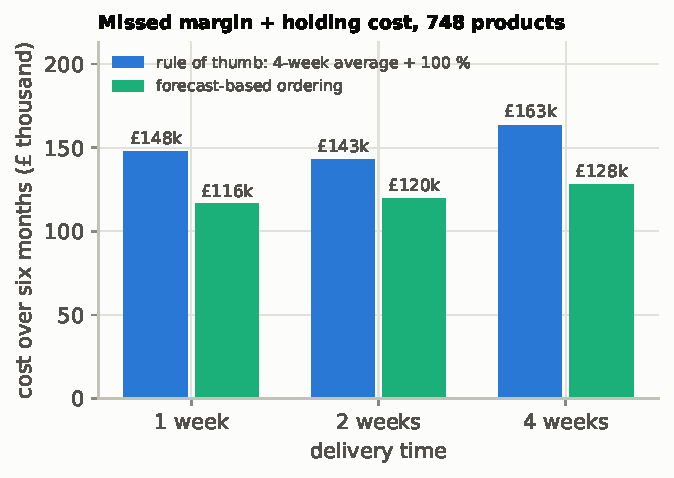
\includegraphics[width=\linewidth]{figures/costs_client.pdf}
\end{minipage}
\footnotetext{Chen, D.\ (2012). \emph{Online Retail II} [Dataset]. UCI Machine Learning Repository. \url{https://doi.org/10.24432/C5CG6D}. Licensed under CC\,BY\,4.0, \url{https://creativecommons.org/licenses/by/4.0/}. Changes: cleaned and aggregated to weekly demand per product.}

\vspace{2pt}
\begin{minipage}[t]{0.48\textwidth}
\head{What you provide}
\begin{itemize}
  \item A sales export: order lines with date, product, quantity and price (ideally two years).
  \item Delivery times per supplier and how often you order.
  \item Margins or purchase prices; your current reorder rule, if you have one.
  \item Optionally current stock levels, to start the order list.
\end{itemize}
\end{minipage}\hfill
\begin{minipage}[t]{0.48\textwidth}
\head{What you get}
\begin{itemize}
  \item A weekly forecast per product, with its range.
  \item A weekly order list (CSV) that your team or system can use directly.
  \item Your current rule against the new policy, simulated on your own history, in your
    currency.
  \item A dashboard to change the service target and see stock and cost move, and a short
    written report.
\end{itemize}
\end{minipage}

\end{document}
